\documentclass[11pt]{exam}

\usepackage{amssymb, amsmath, amsthm, mathrsfs, multicol, graphicx}
\usepackage{tikz}


\def\d{\displaystyle}
\def\?{\reflectbox{?}}
\def\b#1{\mathbf{#1}}
\def\f#1{\mathfrak #1}
\def\c#1{\mathcal #1}
\def\s#1{\mathscr #1}
\def\r#1{\mathrm{#1}}
\def\N{\mathbb N}
\def\Z{\mathbb Z}
\def\Q{\mathbb Q}
\def\R{\mathbb R}
\def\C{\mathbb C}
\def\F{\mathbb F}
\def\A{\mathbb A}
\def\X{\mathbb X}
\def\E{\mathbb E}
\def\O{\mathbb O}
\def\pow{\mathscr P}
\def\inv{^{-1}}
\def\nrml{\triangleleft}
\def\st{:}
\def\~{\widetilde}
\def\rem{\mathcal R}
\def\iff{\leftrightarrow}
\def\Iff{\Leftrightarrow}
\def\and{\wedge}
\def\And{\bigwedge}
\def\AAnd{\d\bigwedge\mkern-18 mu\bigwedge}
\def\Vee{\bigvee}
\def\VVee{\d\Vee\mkern-18 mu\Vee}
\def\imp{\rightarrow}
\def\Imp{\Rightarrow}
\def\Fi{\Leftarrow}



\def\circleA{(-.5,0) circle (1)}
\def\circleAlabel{(-1.5,.6) node[above]{$A$}}
\def\circleB{(.5,0) circle (1)}
\def\circleBlabel{(1.5,.6) node[above]{$B$}}
\def\circleC{(0,-1) circle (1)}
\def\circleClabel{(.5,-2) node[right]{$C$}}
\def\twosetbox{(-2,-1.5) rectangle (2,1.5)}
\def\threesetbox{(-2,-2.5) rectangle (2,1.5)}


\def\bar{\overline}

%\pointname{pts}
\pointsinmargin
\marginpointname{pts}
\marginbonuspointname{ bns pts}

\addpoints
\pagestyle{headandfoot}
%\printanswers


% \firstpageheader{MATH 228}{\bf\large Learning Target Quiz}{Spring 2024}
\header{MATH 131}{\bf\large Learning Target 1 Quiz}{Fall 2025}
\runningfooter{}{}{Version \version}
\extrafootheight{-.45 in}



\begin{document}
\def\version{A}
%space for name
\noindent {\large\bf Name:} \underline{\hspace{2.5 in}}
\vskip 1em




\begin{questions}
  \question The distance $s(t)$ traveled by a bicycle (in feet) after $t$ seconds is given by the function with graph and table below. 
  \begin{multicols}{2}

    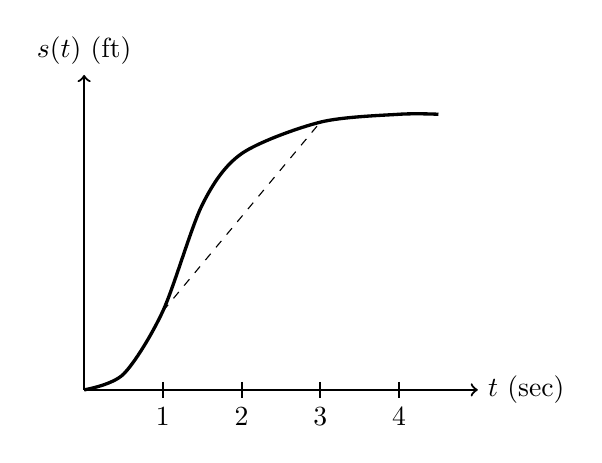
\begin{tikzpicture}
      % Axes:
      \draw[thick, ->] (0,0) -- (0,4) node[above] {$s(t)$ (ft)};
      \draw[thick, ->] (0,0) -- (5,0) node[right] {$t$ (sec)};
      \foreach \x in {1,2,3,4} \draw[thick] (\x,.1) -- (\x,-.1) node[below] {$\x$};
      \draw[very thick] plot[smooth, tension=.5] coordinates {(0,0) (0.5, 0.2) (1,1) (1.5,2.35) (2,3) (3,3.4) (4,3.5) (4.5,3.5)};
      \draw[dashed] (1,1) -- (3,3.4);
    \end{tikzpicture}

    \columnbreak
~
    \vfill

    \begin{tabular}{c|c}
      $t$ (sec) & $s(t)$ (ft) \\
      \hline
      0 & 0 \\
      1 & 10 \\
      2 & 30 \\
      3 & 34 \\
      4 & 35
    \end{tabular}
    \vfill
    \vfill
~
  \end{multicols}
  \begin{parts}
    \part Find the average velocity of the bicycle between second 1 and second 3.
    \vfill
    \part Was the bicycle's instantaneous velocity at second 1 more than or less than its average velocity between second 1 and second 3?  Explain using either the graph or the table above.
    \vfill
  \end{parts}


\end{questions}



\newpage

\def\version{B}
%space for name
\noindent {\large\bf Name:} \underline{\hspace{2.5 in}}
\vskip 1em




\begin{questions}
  \question The height $s(t)$ of a skydiver  (in feet) after $t$ seconds is given by the function with graph and table below. 
  \begin{multicols}{2}

    \begin{tikzpicture}
      % Axes:
      \draw[thick, ->] (0,0) -- (0,5.3) node[above] {$s(t)$ (ft)};
      \draw[thick, ->] (0,0) -- (5,0) node[right] {$t$ (sec)};
      \foreach \x in {1,2,3,4} \draw[thick] (\x,.1) -- (\x,-.1) node[below] {$\x$};
      \draw[very thick, domain=0:2] plot[smooth, tension=.5] (\x, {-\x^2 + 5});
      \draw[very thick, domain=2:4] plot[smooth, tension=.5] (\x, {-0.5*\x + 2});
      \draw[dashed] (1,4) -- (3,0.5);
    \end{tikzpicture}

    \columnbreak
~
    \vfill

    \begin{tabular}{c|c}
      $t$ (sec) & $s(t)$ (ft) \\
      \hline
      0 & 10,000 \\
      1 & 8,000 \\
      2 & 2,000 \\
      3 & 1,000 \\
      4 & 0
    \end{tabular}
    \vfill
    \vfill
~
  \end{multicols}
  \begin{parts}
    \part Find the average velocity of the skydiver second 1 and second 3.
    \vfill
    \part Was the \emph{average} velocity of the skydiver between second 1 and second 3 more than or less than the \emph{instantaneous} velocity at second 3?  Explain using either the graph or the table above.
    \vfill
  \end{parts}
\end{questions}

\newpage

\def\version{C}
%space for name
\noindent {\large\bf Name:} \underline{\hspace{2.5 in}}
\vskip 1em

\begin{questions}
  \question The distance $s(t)$ traveled by a train (in meters) after $t$ minutes is given by the function with graph and table below.
  \begin{multicols}{2}

    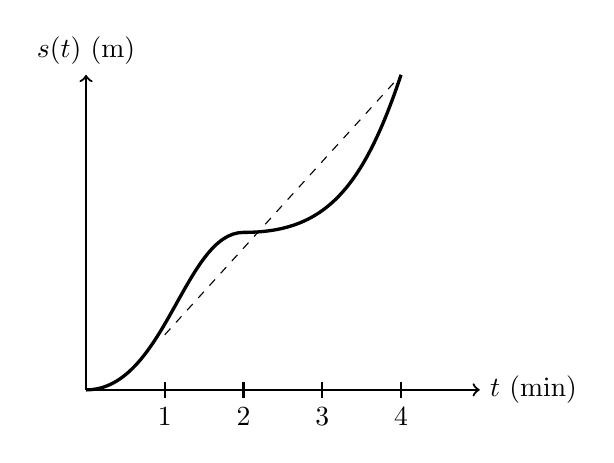
\begin{tikzpicture}
      % Axes:
      \draw[thick, ->] (0,0) -- (0,4) node[above] {$s(t)$ (m)};
      \draw[thick, ->] (0,0) -- (5,0) node[right] {$t$ (min)};
      \foreach \x in {1,2,3,4} \draw[thick] (\x,.1) -- (\x,-.1) node[below] {$\x$};
      \draw[very thick] (0,0) .. controls (1,0) and (1.25,2) .. (2,2) .. controls (3,2) and (3.5, 2.5) .. (4,4);
      \draw[dashed] (1,.7) -- (4,4);
    \end{tikzpicture}

    \columnbreak
~
    \vfill

    \begin{tabular}{c|c}
      $t$ (min) & $s(t)$ (m) \\
      \hline
      0 & 0 \\
      1 & 500 \\
      2 & 800 \\
      3 & 1000 \\
      4 & 1500
    \end{tabular}
    \vfill
    \vfill
~
  \end{multicols}
  \begin{parts}
    \part Find the average velocity of the train between minute 1 and minute 4.
    \vfill
    \part Was the \emph{average} velocity of the train between minute 1 and minute 4 more than or less than the \emph{instantaneous} velocity at minute 2?  Explain using either the graph or the table above.
    \vfill
  \end{parts}
\end{questions}


\newpage

\def\version{D}
%space for name
\noindent {\large\bf Name:} \underline{\hspace{2.5 in}}
\vskip 1em

\begin{questions}
  \question The height $s(t)$ of a model rocket (in feet) after $t$ seconds is given by the function with graph and table below.
  \begin{multicols}{2}

    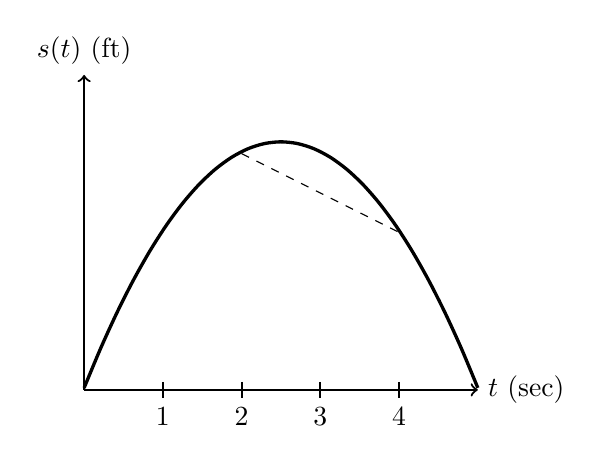
\begin{tikzpicture}
      % Axes:
      \draw[thick, ->] (0,0) -- (0,4) node[above] {$s(t)$ (ft)};
      \draw[thick, ->] (0,0) -- (5,0) node[right] {$t$ (sec)};
      \foreach \x in {1,2,3,4} \draw[thick] (\x,.1) -- (\x,-.1) node[below] {$\x$};
      \draw[very thick, domain=0:5] plot[smooth] (\x, {-.5*(\x-2.5)^2 + 3.15});
      \draw[dashed] (2,3) -- (4,2);
    \end{tikzpicture}

    \columnbreak
~
    \vfill

    \begin{tabular}{c|c}
      $t$ (sec) & $s(t)$ (ft) \\
      \hline
      0 & 0 \\
      1 & 20 \\
      2 & 30 \\
      3 & 30 \\
      4 & 20
    \end{tabular}
    \vfill
    \vfill
~
  \end{multicols}
  \begin{parts}
    \part Find the average velocity of the rocket between second 2 and second 4.
    \vfill
    \part Was the \emph{average} velocity of the rocket between second 2 and second 4 more than or less than the \emph{instantaneous} velocity at second 2?  Explain using either the graph or the table above.
    \vfill
  \end{parts}
\end{questions}


\newpage

\def\version{E}
%space for name
\noindent {\large\bf Name:} \underline{\hspace{2.5 in}}
\vskip 1em

\begin{questions}
  \question The height $s(t)$ of a model rocket (in feet) after $t$ seconds is given by the function with graph and table below.
  \begin{multicols}{2}

    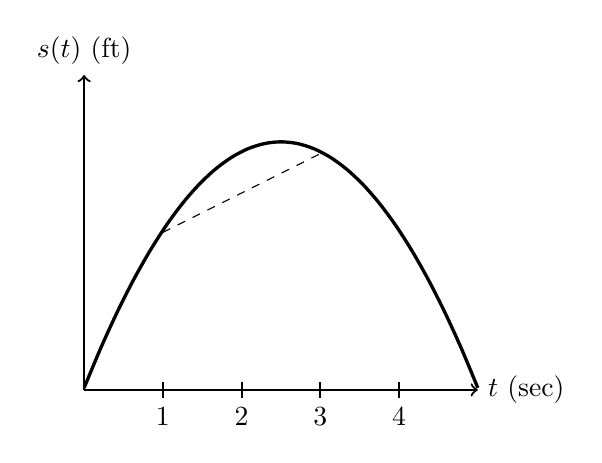
\begin{tikzpicture}
      % Axes:
      \draw[thick, ->] (0,0) -- (0,4) node[above] {$s(t)$ (ft)};
      \draw[thick, ->] (0,0) -- (5,0) node[right] {$t$ (sec)};
      \foreach \x in {1,2,3,4} \draw[thick] (\x,.1) -- (\x,-.1) node[below] {$\x$};
      \draw[very thick, domain=0:5] plot[smooth] (\x, {-.5*(\x-2.5)^2 + 3.15});
      \draw[dashed] (1,2) -- (3,3);
    \end{tikzpicture}

    \columnbreak
~
    \vfill

    \begin{tabular}{c|c}
      $t$ (sec) & $s(t)$ (ft) \\
      \hline
      0 & 0 \\
      1 & 25 \\
      2 & 40 \\
      3 & 40 \\
      4 & 25
    \end{tabular}
    \vfill
    \vfill
~
  \end{multicols}
  \begin{parts}
    \part Find the average velocity of the rocket between second 1 and second 3.
    \vfill
    \part Was the \emph{average} velocity of the rocket between second 1 and second 3 more than or less than the \emph{instantaneous} velocity at second 1?  Explain using either the graph or the table above.
    \vfill
  \end{parts}
\end{questions}

\end{document}
